\documentclass[a4paper,12pt]{article}

\author{\textbf{Софиа Белен Лопес Висенс}\\Группа Б02-903\\ \large Московский физико-технический институт}
\title{Задача: Численное дифференцирование: конечные разности}
\date{17.09.2021}

\usepackage[margin=0.9in]{geometry}
\usepackage{graphicx}
\usepackage{float}
\usepackage[utf8]{inputenc}
\usepackage[T2A]{fontenc}
\usepackage{textcomp}
\usepackage{amsmath, amssymb}
\usepackage{siunitx}
\usepackage{xcolor}

\begin{document}
\maketitle

Пусть \(f(x) = x + \cos x\).
Найдём \(f''(x)\) сначала схемой первой порядка и 
затем схемой второго порядка точности.

\section{Схема 1-го порядка: }

\[
    f_i''(x) = af_{i-2} + bf_{i - 1} + cf_i
\] 

\[
    f_i''(x) = af(x - 2h) + bf(x - h) + cf(x)
\] 

\begin{align*}
    f'' &= a \left(f - 2h f' + \frac{4h^2}{2}f''
    - \frac{8h^3}{6}f'''
    + \frac{16h^4}{24} f^{IV} + o (h^4) \right) \\
        &+ b \left(f - h f' + \frac{h^2}{2}f''
    - \frac{h^3}{6}f'''
    + \frac{h^4}{24} f^{IV} + o (h^4) \right) \\
        &+ cf
\end{align*}

\[
\begin{cases}
    a + b + c = 0 \\
    -2a - b = 0 \\
    4 h^2 a + h^2 b = 2 \\
\end{cases}
\iff
\begin{cases}
    a + b + c = 0 \\
    b = -2a \\
    4h^2 a - 2h^2 a = 2
\end{cases}
\iff
\begin{cases}
    a = \frac{1}{h^2} \\
    b = -\frac{2}{h^2} \\
    c = \frac{1}{h^2}
\end{cases}
\] 

\[
    f_i''(x) = \frac{f_{i - 2} - 2 f_{i - 1} + f_{i} }{h^2}
    - \frac{8h}{6} f'''
    + \frac{2h}{6} f'''
    + o(h)
\] 

\[
    f_i''(x) = \frac{f_{i - 2} - 2 f_{i - 1} + f_{i} }{h^2}
    - hf'''
    + \underbrace{o(h)}
\] 

\[
    f_i''(x) = \frac{f_{i - 2} - 2 f_{i - 1} + f_{i} }{h^2}
    - h f'''(\xi), \qquad \xi \in [x - 2h, x]
\] 

\[
    \boxed{f_i''(x) = \frac{f_{i - 2} - 2 f_{i - 1} + f_{i} }{h^2}}
\] 

\[
    \delta = |h f'''(\xi)|
    \le  h M_3, \qquad M_3 = \max_{x \in [x - 2h, x]}
    |f'''(x)|
\] 

\[
    \varepsilon_c = \Delta \left( \frac{f_{i - 2}
- 2 f_{i - 1} + f_{i} }{h^2} \right) 
= \frac{1}{h^2} \left( \Delta f + 2 \Delta f
+ \Delta f \right) 
= \frac{4E}{h^2}
\] 

\[
    \varepsilon'_h = \left( hM_3
    + \frac{4E}{h^2} \right)'_h
    = M_3 - \frac{8E}{h^3} = 0
\] 

\(E = 2^{-53}\), \(M_3 = 1\)

\[
   \boxed{h_{opt} = \sqrt[3]{\frac{8E}{M_3}} 
    \approx 9.28 \cdot 10^{-6}} 
\] 

\begin{figure}[htpb]
    \centering
    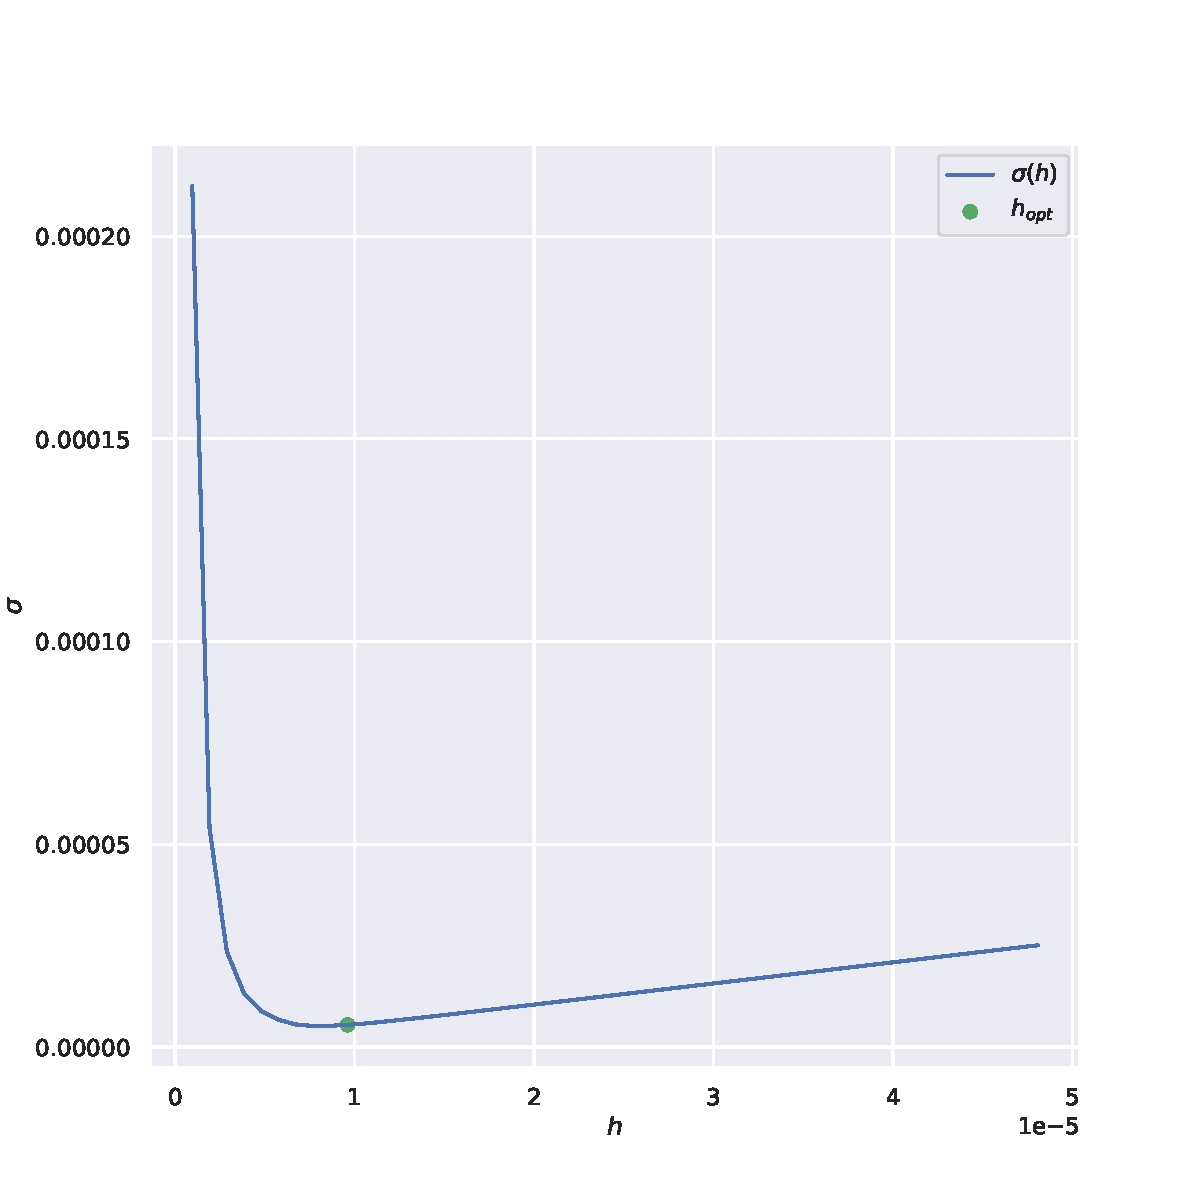
\includegraphics[width=0.8\textwidth]{../img/graph1.pdf}
    \caption{Погрешность метода 1-го порядка в
    зависимости от шага интегрирования}
\end{figure}

\section{Схема 2-го порядка: }

\[
    f_i''(x) = a f_{i - 1} + bf_i + c f_{i + 1}
\] 

\begin{align*}
    f'' &= a \left(f - h f' + \frac{h^2}{2}f''
    - \frac{h^3}{6}f'''
    + \frac{h^4}{24} f^{IV} + o (h^4) \right) \\
        & + bf \\
        & + c \left( f + hf' + \frac{h^2}{2}f''
    + \frac{h^3}{6}f'''
    + \frac{h^4}{24} f^{IV} + o(h^4) \right)
\end{align*}

\[
\begin{cases}
    a + b + c =0 \\
    -a + c = 0 \\
    a \frac{h^2}{2} + c \frac{h^2}{2} = 1
\end{cases}
\implies \begin{cases}
    a = c = \frac{1}{h^2} \\
    b = - \frac{2}{h^2}
\end{cases}
\] 

\[
    f_i'' = \frac{f_{i - 1} - 2f_i + f_{i + i} }{h^2}
    - \frac{h}{6} f'''
    + \frac{h}{6} f'''
    + 2 \cdot \frac{h^2}{24} f^{IV}
    + \underbrace{o(h^2)}
\] 

\[
    f_i'' = \frac{f_{i - 1} - 2f_i + f_{i + i} }{h^2}
    + \frac{h^2}{12} f^{IV}(\xi), \qquad
    \xi \in [x - h, x + h]
\] 

\[
   \boxed{f_i'' = \frac{f_{i - 1} - 2f_i + f_{i + i} }{h^2}} 
\] 

\[
    \delta = \left| \frac{h^2}{12}f^{IV}(\xi) \right| 
    \le  \frac{h^2M_4}{12}, \qquad
    M_4 = \max_{ \xi \in [x - h, x + h]} f(\xi)
\] 

\[
    \varepsilon_C = \Delta \left( \frac{f_{i - 1}
    - 2f_i + f_{i + i} }{h^2} \right) 
    = \frac{4\Delta f}{h^2} \le  \frac{4E}{h^2}
\] 

\[
    \varepsilon'_h = \left( \frac{h^2M_4}{12}
    + \frac{4E}{h^2}\right)'_h = \frac{M_4h}{6}
    - \frac{8E}{h^3} = 0
\] 

\[
  \boxed{h_{opt} = \sqrt[4]{\frac{48 E}{M_4}} 
    \approx 2.63 \cdot 10^{4}}  
\] 

\begin{figure}[htpb]
    \centering
    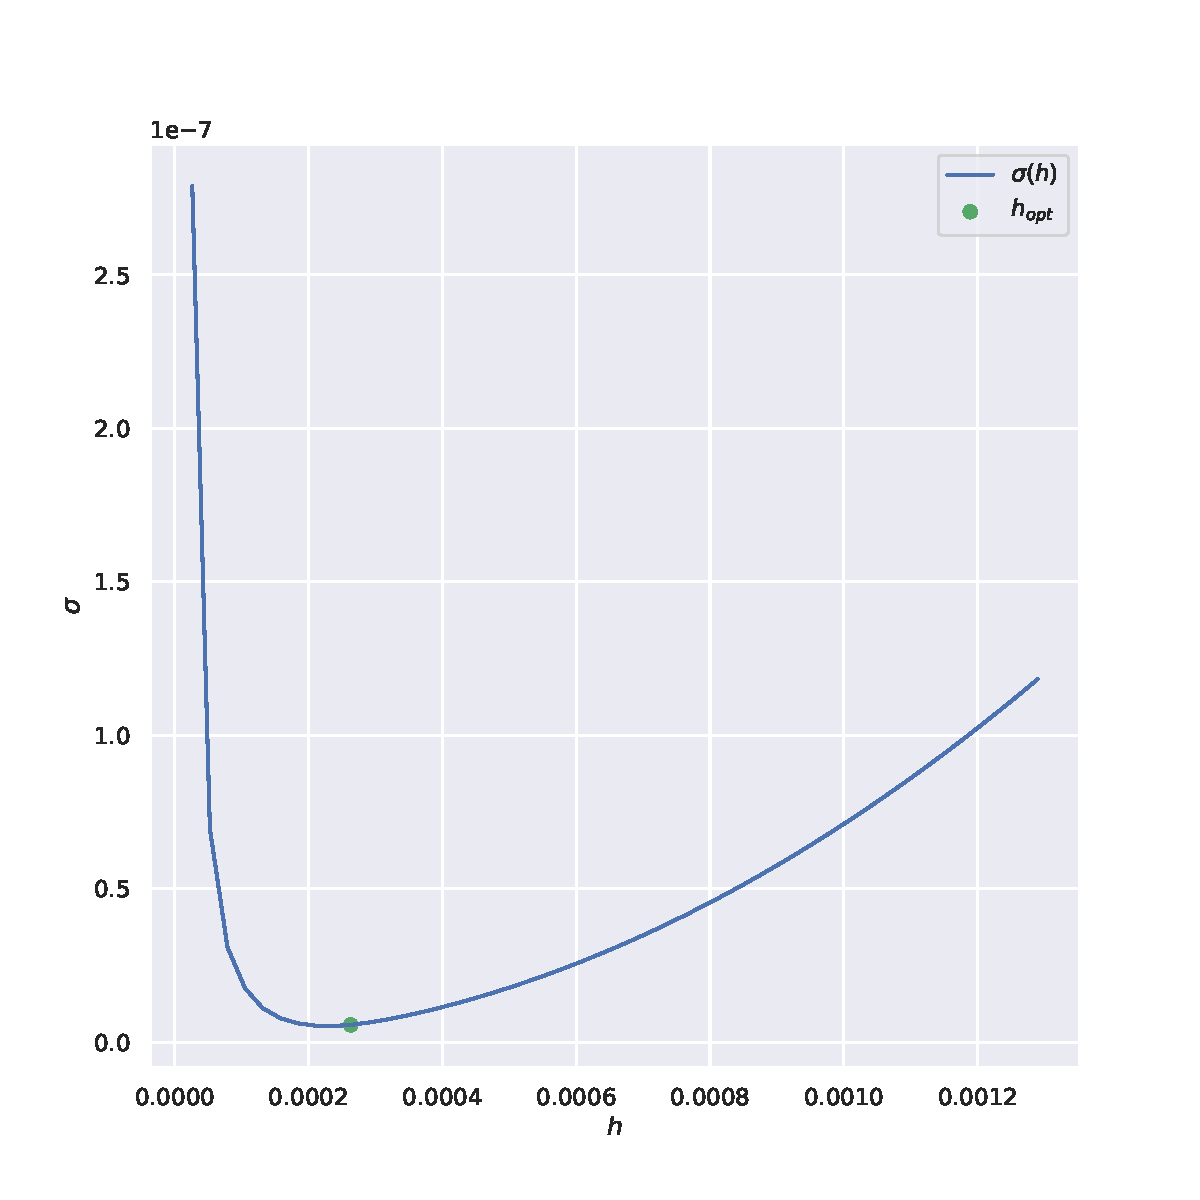
\includegraphics[width=0.8\textwidth]{../img/graph2.pdf}
    \caption{Погрешность метода 2-го порядка в
    зависимости от шага интегрирования}
\end{figure}
    
\end{document}
